\documentclass[12pt, a4paper]{report}
\usepackage[pdftex]{graphicx} %for embedding images
\graphicspath{ {./img/} } %the path to the images
\usepackage[,italian, english]{babel}
\usepackage{url} %for proper url entries
% \usepackage[bookmarks, colorlinks=false, pdfborder={0 0 0}, pdftitle={<pdf title here>}, pdfauthor={<author's name here>}, pdfsubject={<subject here>}, pdfkeywords={<keywords here>}]{hyperref} %for creating links in the pdf version and other additional pdf attributes, no effect on the printed document
%\usepackage[final]{pdfpages} %for embedding another pdf, remove if not required

\begin{document}
\renewcommand\bibname{References} %Renames "Bibliography" to "References" on ref page


\begin{titlepage}

\begin{center}

\Large \textbf {Programmazione Concorrente e Distribuita - Assigment 03}\\%\\[0.5in]
\vspace{1em}%
\vfill
Leonardo Randacio


Filippo Gurioli


Andrea Biagini
\vspace{1em}
\vfill
{\bf Università di Bologna \\ Scienze e Ingegneria Informatiche}\\[0.5in]

       
\vfill
\today

\end{center}

\end{titlepage}


\tableofcontents
\listoffigures
\listoftables

\newpage
\pagenumbering{arabic} %reset numbering to normal for the main content

\chapter{Analysis}
The goal is to create a Cooperative Sudoku exploiting the Croquet.io Framework.
%
The game is a cooperative version of the classic Sudoku game. The game can be played by any number of players, each player can see the board and the numbers placed by the other players. The game is won when the board is completed.
Each player can also be able to see the other players' cursors, and have the capability to exit and join different games at any time.

\section{Task Decomposition}
The game can be decomposed in the following tasks:
\begin{itemize}
    \item \textbf{create game}: create a new game
    \item \textbf{join game}: join an existing game
    \item \textbf{exit game}: exit the current game
    \item \textbf{place number}: place a number in the board
    \item \textbf{move cursor}: move the cursor in the board
\end{itemize}
Each task can be executed by any player at any time.

\section{Data Decomposition}
The game is composed by a board, a set of players, a set of cursors and a set of numbers placed in the board.

\section{Dependency Analysis}
There is different dependency level. The first and most visible one is between tasks that belong to different parts of the game. That is the dependency between the place number and move tasks and the create/join/exit task. The second level of dependency is between all tasks that belong to the same part of the game. For example, the place number task is dependent on the move cursor task; the join and task is dependent on the create task.\\

\chapter{Design}
Exploiting Croquet.io Framework, the game is designed as a set of objects that communicate with each other via messages. Each object can perform every task of the game and the execution of a task is fired by a message sent to the object. In order to let all be in synch with the game state, Croquet.io provides a shared state that is updated by the objects. The shared state is a javascript class that is ensured to be the same on all objects. That is, when an object updates the shared state, the change is propagated to all the other objects.

TODO: potrei andare avanti ad oltranza, capire quale è il livello giusto di astrazione di cui parlare qui

\section{Architecture}
Since the game should provide both the capabilities to create and join games and to play the game, the architecture is divided in two macroparts: the lobby and the game. The lobby is the part of the game where the player can create or join a game. The game is the part of the game where the player can play the game (and exit). Each user is represented by an object as defined earlier.

\begin{figure}
    \centering
    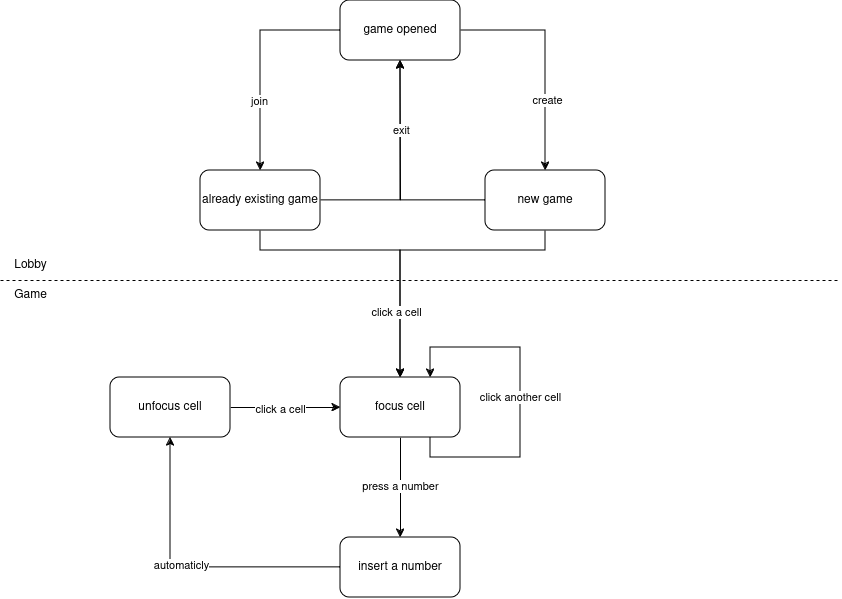
\includegraphics[scale=0.5]{part2a-states.png}
    \caption{UML diagram exposing all possible states of the game and how they are related.}
\end{figure}

\begin{figure}
    \centering
    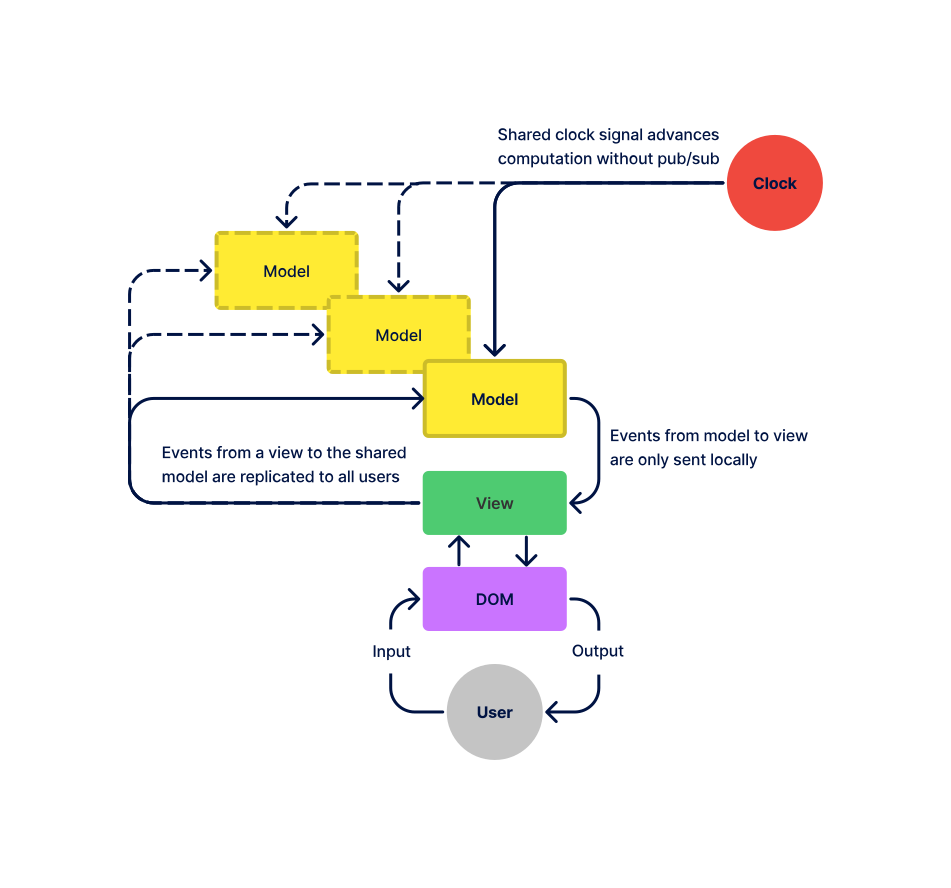
\includegraphics[scale=0.5]{croquet_overview.png}
    \caption{Croquet.io overview on how the system is structured.}
\end{figure}

\bibliographystyle{plain}
\bibliography{References}

\end{document}